\eandmchapter{Algorithmic Specified Complexity}{Algorithmic Specified Complexity}{Winston Ewert, William A. Dembski, and Robert J. Marks II}{Baylor University\\Discovery Institute}

\index{information!see{complexity}}

\begin{abstract}
\index{complexity!metrics!Kolmogorov complexity}
\index{complexity!metrics!conditional Kolmogorov complexity}
As engineers we would like to think that we produce something different from that of a chaotic system. The Eiffel tower is  fundamentally different from the same components lying in a heap on the ground. Mt. Rushmore is fundamentally  different from a random mountainside. But we lack a good method for quantifying this idea. This has led some to reject the idea that we can detect engineered or designed systems. Various methods have been proposed each of which has
various faults. Some have trouble distinguishing noise from data, some are subjective, etc. We propose to use conditional Kolmogorov complexity to measure the degree of specification of an object. The Kolmogorov complexity of an object, is the length of the shortest computer program required to describe that object. Conditional Kolmogorov complexity is Kolmogorov complexity, with access to a  context. The program can extract information from the context in a variety of ways allowing more compression. The more compressible an object is the more we may deem the object specified. Random noise is  incompressible, and so compression indicates that the object is not simply random noise. 
We hope this model launches further dialog on use of conditional Kolmogorov complexity in the measurement of specified complexity.
\end{abstract}

\section{Introduction}
\index{Mount Rushmore}
Intuitively, humans identify objects such as the carved faces at Mount Rushmore as qualitatively different from that of a random mountainside.
However, quantifying this concept is an objective manner has proved difficult.
Both mountainsides are made up of the same material components.
They are both subject to the same physical forces, and will react the same to almost all physical tests.
Yet, there does appear to be something quite different about Mount Rushmore.
There is a special something about carved faces that separates it from the rock it is carved in.

\index{information}
This ``special something'' is information.
Information is what distinguishes an empty hard disk from a full one.
Information is the difference between random scribbling and carefully printed prose.
Information is the difference between car parts strewn over a lawn, and a working truck.

While humans operate using an intuitive concept of information, attempts to develop a theory of information has thus far fallen short of the intuitive concept.
\index{Shannon information|see{complexity, metrics, Shannon information}}
\index{complexity!metrics!Shannon information}
Claude Shannon developed what its today known as Shannon information theory \citep{Shannon1948}.
Shannon's concern was studying the problem of communication, that of sending information from one point to another.
However, Shannon explicitly avoided the question of the meaningfulness of the information being transmitted, thus not quite capturing the concept of information as we are defining it.
In fact, under Shannon's model a random signal has the highest amount of information, the precise opposite of the intuitive concept.

\index{algorithmic information theory}
Another model of information is that of algorithmic information theory \citep{Chaitin1966, Solomonoff1960, Kolmogorov1968a}.
\index{Kolmogorov complexity|see{complexity, metrics, Kolmogorov complexity}}
\index{complexity!metrics!Kolmogorov complexity}
Techniques such as Kolmogorov complexity measure the complexity of an object as the minimum length computer program required to recreate the object; Chaitin refers to such minimum length programs as \textit{elegant} \citep{Chaitin2002}.
As with Shannon information, random noise is the most complex because it requires a long computer program to describe.
In contrast, simple patterns are not complex because a short computer program can describe the pattern.
But neither simple patterns or random noise are what we think of as information.
As with Shannon information, there is a disconnect between Kolmogorov complexity and conceptual information.

Other models are based on algorithmic information theory, but also take in account the computational resources required for the programs being run.
\index{complexity!metrics!Levin complexity}
Levin complexity adds the log of the execution time to the complexity of the problem \citep{Levin1976}.
\index{complexity!metrics!logical depth}
\index{logical depth|see{complexity, metrics, logical depth}}
\textit{Logical depth}, on the other hand, is concerned with the execution time of the shortest program \citep{Bennett1988}.
There is a class of objects which are easy to describe but expensive to actually produce.
It is argued \citep{Bennett1988} that objects in this class must have been produced over a long history.
Such objects are interesting, but do not seem to capture all of what we consider to be the intuitive concept of information.
English text or Mount Rushmore correspond to what we think of as information, but its not clear that they can be most efficiently described as long running programs.

\index{complexity!metrics!specified complexity}
\index{specified complexity|see{complexity, metrics, specified complexity}}
\index{chance}
\index{necessity}
\index{agency}
\index{intelligence}
One approach to information is the \textit{specified complexity} as expressed by Dembski \citep{Dembski1998}.
Dembski's concern is that of detecting design, the separation of that which can be explained by chance or necessity from that which is the product of intelligence. 
In order to infer design, and object must be both complex and specified.
Complexity refers essentially to improbability.
The probability of any given object depends on the chance hypothesis proposed to explain it.
Improbability is a necessary but not sufficient condition for rejecting a chance hypothesis.
Events which have a high probability under a given chance hypothesis do not give us reason to reject that hypothesis.

\index{specification}
Specification is defined as conforming to an independently given pattern.
The requirement for the pattern to be independent of the object being investigated is fundamental.
Given absolute freedom of pattern selection, any object can be made specified by selecting that object as the pattern.
It is not impressive to hit a bullseye if the bullseye is painted on after the arrow has hit the wall.
It is impressive to hit the bullseye if the bullseye was painted before the arrow was fired.

\index{self-replication}
Investigators are often not in the position of being able to choose the target prior to investigating the object.
Consider the example of life.
Life is a self-replicating process, and it would seem that an appropriate specification would be self-replication.
Self-replication is what makes life such a fascinating area of investigation as compared to rocks.
We know about self-replication \emph{because of} our knowledge of life, not as an independent fact.
Therefore it does not qualify as an independent specification.
If we did not already have examples of self-replicating entities, we would not have picked as the specification.

The same is true of almost any specification in biology.
It is tempting to consider flight a specification, but we would only be defining the pattern of flight because we have seen flying animals.
As with life in general, specific features in biology cannot be specified independently of the objects themselves.

\index{specification|(}
\index{complexity!metrics!conditional Kolmogorov complexity}
\index{complexity!metrics!algorithmic specified complexity}
\index{algorithmic specified complexity|see{complexity, metrics, algorithmic specified complexity}}
The concept of specification has been criticized for being imprecisely defined and unquantifiable.
It is also charged that the maintaining the independence of the patterns is difficult.
But specification has been defined in a mathematically rigorous manner in several different ways \citep{Dembski1998, Dembski2002, Dembski2005a}.
Kolmogorov complexity, or a similar concept, is a persistent method used in this definitions.
Our goal is to present and defend a simple measure of specification that clearly alleviates these concerns.
Towards this end, we propose to use \textit{conditional Kolmogorov complexity} to quantify the degree of specification in an object.
Combining this with the complexity, we can quantify the specified complexity as \textit{algorithmic specified complexity}.

As noted, Kolmogorov complexity has been suggested as a method for measuring specification.
The novelty in method presented in this paper is the use of conditional Kolmogorov complexity.
However, this paper also elucidates a number of examples of algorithmic compressibility demonstrating wider applicability then is often realized.

\section{Method}

\subsection{Kolmogorov}

\index{complexity!metrics!Kolmogorov complexity|(}
Kolmogorov complexity is a method of measuring information.
It is defined as the minimum length computer program, in bits, required to produce a binary string.
\begin{equation}
    K(X) = \min_{U(p,) = X \mid p \in P} |p|
\end{equation} where
\begin{itemize}
    \item $K(X)$ is the Kolmogorov complexity of X
    \item $P$ is the set of all possible computer programs
    \item $U(p,)$ is the output of program $p$ run without input
\end{itemize}
The definition is given for producing binary strings.

Kolmogorov complexity measures the degree to which a given bitstring follows a pattern.
The more a bitstring follows a pattern, the shorter the program required to reproduce it.
In contrast, if a bitstring exhibits no patterns, it is simply random, and a much longer program will be required to produce it.

\index{bitstrings}
Consider the example of a random binary string, {\tt 100100000010100000001010}.
It can be produced by the following Python program:
\begin{verbatim}
    print '100100000010100000001010'
\end{verbatim}
In contrast, we have the string, {\tt 000000000000000000000000}, which can be produced by
\begin{verbatim}
    print '0' * 24
\end{verbatim}
Both strings are of the same length, but the string following a pattern requires a shorter program to produce.
Thus we have a technique for measuring the degree to which a binary string follows a pattern.

Specification is defined as following an independently given pattern.
Kolmogorov complexity gives us the ability to precisely define and quantify the degree to which a binary string follows a pattern.
Therefore, it seems plausible that we can measure specification using Kolmogorov complexity.
The more compressible a bitstring, the more specified it is.

However, Kolmogorov complexity seems unable to capture the entirety of what is intended by specification.
Natural language text is not reducible to a simple pattern; however, it is an example of what we'd consider specification.
The design of an electronic circuit should also be specified, but it is not reducible to a simple pattern.
In fact, the cases of specification that Kolmogorov complexity seems able to capture are limited to objects which exhibit some very simple pattern.
But these are not the objects of most interest in terms of specification.
\index{complexity!metrics!Kolmogorov complexity|)}

\index{complexity!metrics!conditional Kolmogorov complexity}
We use an extension of Kolmogorov complexity known as {\it conditional Kolmogorov complexity} \citep{Kolmogorov1968}.
The program now has access to additional data as its input.
\begin{equation}
    K(X|Y) = \min_{U(p,Y) = X \mid p \in P} |p|
\end{equation} where $U(p,Y)$ is the output of running program $p$ with input $Y$.
The input provides additional data to the program.
As a result, the program is no longer restricted to exploiting pattern in the desired output, but can take advantage of the information provided by the input.
\index{context}
Henceforth, we will refer to this input as the {\it context}.

The use of context allows the measure to capture a broader range of specifications.
It is possible to describe many bitstrings by combining a short program along with the contextual information.
A useful range of specifications can be captured using this technique.
\index{specification|)}

\subsection{Algorithmic Specified Complexity}

\index{complexity!metrics!algorithmic specified complexity|(}
To combine the measurement of specification and complexity, we use the following formula for algorithmic specified complexity (ASC).
\begin{equation}
    \label{ASC}
    A(X,C,p) = -\log p(X) - K(X|C)
\end{equation} where
\begin{itemize}
    \item $X$ is the bitstring being investigated
    \item $C$ is the context as a bitstring
    \item $p$ is the probability distribution which we suppose X to have been selected from
    \item $p(X)$ is the probability of X occurring according to the chance hypothesis under consideration
\end{itemize}
Since high compressibility corresponds to specification, we subtract the compressed length of the string.
Thus high improbability counts for specified complexity, but incompressible strings count against it.

For this number to become large requires X to be both complex, (i.e. improbable), and specified, (i.e. compressible).
Failing on either of these counts will produce a low or negative value.
Since Kolmogorov complexity can, at best, be upper bounded, the ASC can, at best, be lower bounded.

At best this measure can reject a given probability distribution.
It makes no attempt to rule out chance based hypothesis in general.
However, it can conclude that a given probability distribution does a poor job in explaining a particular item.
The value of ASC gives a measure of the confidence we can have in rejecting a chance hypothesis.

\subsection{Functionality}

\index{functionality}
Perhaps the most interesting form of specification is that of functionality.
It is clear that machines, biological structures, and buildings all have functionality.
But quantifying that in an objective manner has proven difficult.
However, ASC gives us the ability to do this.

Any machine can be described, in part, by tests that it will pass.
You can test the functionality of a car by seeing whether it accelerates when the gas or brake pedals are pushed.
You can test the functionality of a cell by seeing whether it self-replicates.
A test, or a number of tests, can be defined to identify the functionality of an object 
The existence of a test gives us the ability to compress the object.
Consider the following pseuocode program:
\begin{verbatim}
counter = 0
for each possible building design
    if building won't fall over
        counter += 1
        if counter == X
             return building design
\end{verbatim} where X is some number.
This program will output the design for a specific building.
Different values of X will produce different buildings.
But any building that will not fall over can be expressed by this program.
It may take a considerable amount of space to encode this number.
However, if few designs are stable, the number will take much less space than required to actually specify the building plans.
Thus the stability of the building plan enables compression, which in turn indicates specification.

Kolmogorov complexity is not limited to exploiting what humans perceive as simple patterns.
It can also capture other aspect such as functionality.
Functionality can be described as passing a test.
As a result functional objects are compressible.

\section{Examples}
\subsection{Natural Language}
\index{English text}
As the first example, consider the sentence: ``the quick brown fox jumps over the lazy dog.''
We can encode this sentence as UTF-32, a system for encoding that allows the encoding of symbols from almost any alphabet.
Since each character takes 32 bits, the message will be encoded as a total of 1376 bits.
In this case, we will take the context to be the English alphabet along with a space.
This is a minimal level of information about the English language.

To specify one of the 27 characters, will require $\log_2 27$ bits. 
To specify the 43 character in the sentence will thus take $43 \log_2 27$ bits.
We also need to record the number of characters at $2 \log_2 43 \approx 10.85$ bits. 
\footnote{A more compact representation for numbers is available. See the $log^*$ method in \citet{Cover2006}.}
Altogether, the bits required to specify the message requires $43 \log_2 27 + 2 \log_2 43 \approx 215.32$ bits. 


However, in order to actually give a bound for Kolmogorov complexity, we must also include the length of the computer program which interprets the bits.
Here is an example computer program in Python which could interpret the message
\begin{verbatim}
    print ''.join(alphabet[index] for index in encoded_message)
\end{verbatim}
This assumes that the alphabet and encoded message are readily available and in form amenable to processing within the language.
It may be that the input has to be preprocessed, which would make the program longer.
Additionally, the length of the program will vary heavily depending on which programming language is used.
However, the distances between different computers and languages only differs by a constant \citep{Cover2006}.
As a result, it is common practice in algorithmic information theory, to discount any actual program length and merely include that length 
as a constant, $c$. 
Consequently, we can express the conditional Kolmogorov complexity as 
\begin{equation}
    \label{kc.alpha}
    K(X|C) \leq 215.32 \mbox{ bits} + c \mbox{.}
\end{equation}
The expression is less than rather than equal, because it is possible that an even more efficient way of expressing the sentence exists.
But we know that at least this efficiency is possible.

The encoded version of the sentence requires 32 bits for each character, giving a total of 1376 bits.
We adopt a simplistic probability model, supposing that each bit is generated by the equivalent of a coin flip.
This means that the complexity, $-\log P(X)$ is 1376 bits.
Using equation~\ref{ASC},
\begin{equation}
    A(X,C,p) = -\log(p) - K(X|C) \geq 1376 \mbox{ bits} - 215.32 \mbox{ bits} - c  = 1160.68 \mbox{ bits} - c \mbox{.}
\end{equation}
This means that we have 1166 bits of algorithmic specified complexity by equation~\ref{ASC}.
Those 1166 bits are a measure of the confidence in rejecting the hypothesis that the sentence was generated by random coin flips.
The large number of bits gives a good indication that is highly unlikely that this sentence was generated by randomly choosing bits.

However, we can also analyze the hypothesis that the sentence was generated by choosing random English letters.
In this case we can calculate the probability of this sentence as
\begin{equation}
    P(X) = \left(\frac{1}{27}\right)^{43} \mbox{.}
\end{equation}
The complexity is then
\begin{equation}
    -\log P(X) = -\log \left(\frac{1}{27}\right)^{43} = 43 \log 27 \approx 204.46 \mbox{ bits.}
\end{equation}
In which case the algorithmic specified complexity becomes
\begin{equation}
    A(X,C,p) = - \log p(X) - K(X|C) \geq 204.46 \mbox{ bits} - 215.32 \mbox{ bits} - c = -10.85 \mbox{ bits} - c \mbox{.}
\end{equation}
The negative bound indicates that we have no reason to suppose that this sentence could not have been generated by a random choice of English letters.
The bound is negative as a result of two factors.
In the specification, $10.85$ bits were required to encode the length.
On the other hand, the probability model assumes a length.
Hence the negative bits indicate information which the probability model had, but was not provided in the context.
Since the only provided context is that of English letters, this is not a surprising result.
We did not identify any sort of pattern beyond that explained by the probability model.

We can also expand the context.
\index{dictionary}
Instead of providing the English alphabet as our context, we provide the word list of the Oxford English Dictionary \citep{Oxford2012}.
In the second edition of that dictionary there were 615,100 word forms defined or illustrated.
For the purpose of the alphabet context, we encode each letter as a number corresponding to that character.
In this case, we can choose a number corresponding to words in the dictionary.
We can thus encode this message:
\begin{equation}
    \label{kc.dict}
    K(X|C) \leq 9 \log_2  615,100 + 2 \log_2 9 + c \approx 179.41 + c \mbox{.}
\end{equation}
Access to the context of the English dictionary allows much better compression than simply the English alphabet as comparing equations~\ref{kc.alpha} and ~\ref{kc.dict} shows.

Using equation~\ref{ASC}, we determine
\begin{equation}
    A(X,C,p) = - \log p(X) - K(X|C) \geq 204.46 \mbox{ bits} - 179.41 \mbox{ bits} - c = 25.05 \mbox{ bits} - c \mbox{.}
\end{equation}
This gives us confidence to say this sentence was not generated by randomly choosing letters from the English alphabet.

It would be possible to adopt a probability model that selected random words from the English language.
Such a probability model would explain all of the specification in the sentence.
It would also be possible to include more information about the English language such that the specification would increase.

This technique depends on the fact that the numbers of words in the English language is much smaller then the number of possible combinations of letters.
If the dictionary contained every possible combination of letters up to some finite length, it would not allow compression, and thus we would not be able to indicate specification.
A language where all possible combinations of letters were valid words could still show specification, but another technique would have to be used to allow compression.

But one could also use a much smaller dictionary.
A dictionary of 10 words would be sufficient to include all the words in this sentence.
The ASC formula would give a much smaller compressed bound:
\begin{equation}
    K(X|C) \leq 9 \log_2 10 + 2 \log_2 9 \approx 36.24 \mbox{ bits.}
\end{equation}
This is a reduction of over 100 bits from equation~\ref{kc.dict}.
This is because it takes about 16 bits less to encode each word when the dictionary is this small.
This is because the sentence is much more closely related to the context.
It requires much less additional information to use the context.

But it is possible to include words not included in the dictionary.
The program would have to fall back on spelling the word one letter at a time.
Only bounds of the ASC can be computed.
It is always possible a better compression exists; i.e.\ the object could be more specified than we realize.

\subsection{Random Noise}
\index{randomness}
While natural language is an example of something that should be specified, random noise is an example of something which should not.
We will calculate the ASC of a random bitstring.
This bitstring will contain 1000 bits, where each bit is assigned with equal probability 1 or 0.
Since randomness is incompressible, calculating the Kolmogorov complexity is easy.
The only way of reproducing a random bitstring is to describe the whole bitstring.
\begin{equation}
    K(X) \leq 2 \log_2 1000 + 1000 + c \approx 1020 \mbox{ bits} + c
\end{equation}
The probability of each bitstring is $2^{-1000}$ and thus the complexity will be 1000 bits.
Calculating the ASC:
\begin{equation}
    A(X,C,p) = - \log p(X) - K(X|C) \geq 1000 \mbox{ bits} - 1020 \mbox{ bits} - c = -20 \mbox{ bits} - c \mbox{.}
\end{equation}
As expected, the ASC is negative, there is no evidence of pattern in the string which are not explained by the probability model.

However, we can also consider the case of a biased distribution.
That is, 1 and 0 are not equally likely.
Instead, a given bit will be one two thirds of the time, while zero only one third of the time.
The entropy of each bit can be expressed as
\begin{equation}
    H(X_i) = - \frac{1}{3} \log_2 \frac{1}{3} - \frac{2}{3} \log_2 \frac{2}{3} \approx 0.6365 \mbox{ bits.}
\end{equation} for any $i$
The entropy of a bit is the number of bits required in an optimal encoding to encode each bit.
This means we can describe the whole sequence as
\begin{equation}
    K(X) \leq 2 \log_2 1000 + 1000*H(X_i) + c \approx 656.5 \mbox{ bits} +c \mbox{.}
\end{equation}
If we adopt the uniform probability model, the complexity is still 1000 bits and
\begin{equation}
    A(X,C,p) = - \log p(X) - K(X|C) \geq 1000 \mbox{ bits} - 656.5 \mbox{ bits} - c = 343.3 \mbox{ bits} -c \mbox{.}
\end{equation}
This random sequence has a high bound of algorithmic specified complexity.
It is important to remember that the ASC bound only serves to measure the plausibility of the random model.
It does not exclude the existence of another more accurate model that explains the data.
In this case, if we use the actual probability model used to generate the message
\begin{equation}
    -\log_2(p) = H(X_i) * 1000 \approx 636.5 \mbox{ bits.}
\end{equation}
and the resulting ASC:
\begin{equation}
    A(X,C,p) = - \log p(X) - K(X|C) \geq 636.5 \mbox{ bits} - 656.5 \mbox{ bits} - c = -20 \mbox{ bits} -c \mbox{.}
\end{equation}
The bound of ASC gives us reason to reject a uniform noise explanation for this data, but not the biased coin distribution.

\index{ballot rigging}
Dembski \citep{Dembski1998} has considered the example of ballot rigging where a political party is almost always given the top billing on the ballot listing candidates.
Since the selection is supposed to be chosen on the basis of a fair coin toss, this is suspicious.
ASC can quantify this situation.
We can describe the outcome by giving the numbers of heads and tails, follow by the same representation as for the biased coin distribution.
\begin{equation}
    K(X) \leq 2 \log X_h + 2 \log X_t + \log {X_t + X_h \choose X_h} + c
\end{equation} where $X_h$ is the number of heads, $X_t$ is the number of tails
We assume a probability model of a fair coin
\begin{equation}
    -\log_2(p) = X_h + X_t \mbox{bits.}
\end{equation}
This gives us:
\begin{align}
    A(X,C,p) &= X_h + X_t - 2 \log X_h -  2 \log X_t - \log {X_t + X_h \choose X_h} - c \nonumber \\
    &= X_h + X_t - \log \left( X_h^2 X_t^2 {X_t + X_h \choose X_h} \right) - c \mbox{.}
\end{align}
\begin{figure}
    \begin{center}
        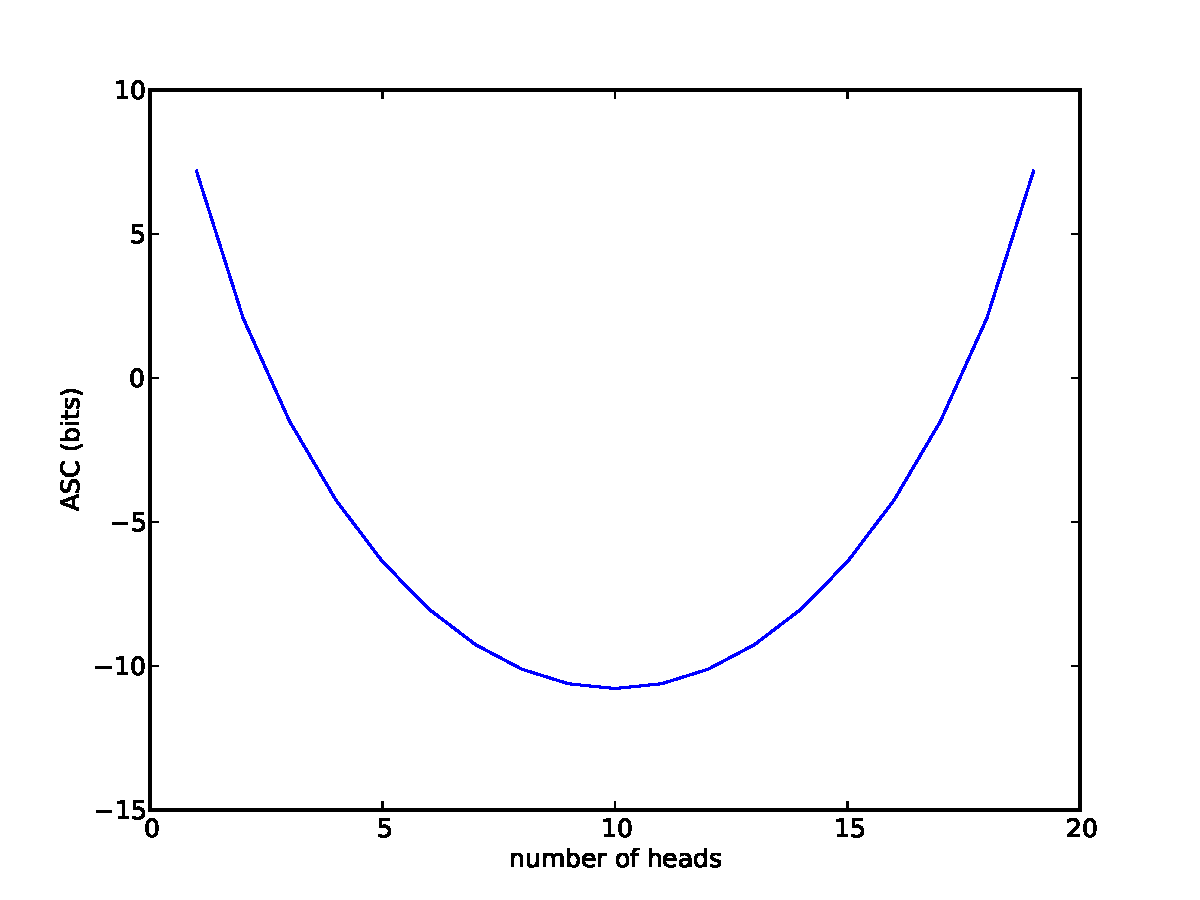
\includegraphics[width=.5\textwidth]{EwertCoin}
    \end{center}
    \caption{ASC for varyingly biased coin sequences and 20 coin tosses}
    \label{fig_coins}
\end{figure}
Figure~\ref{fig_coins} shows the result of plotting this equation for varying numbers of head and tails given 20 coin tosses.
As expected, for either high numbers of tails or high number of heads, the bound of ASC is high.
However, for an instance which looks like a random sequence, the ASC is minimized.


\subsection{Playing Cards}

\index{poker}\index{cards}
Another interesting case is that of playing cards for poker.
In playing cards if the distribution is not uniform; somebody is likely cheating.
For the purpose of investigating card hands, we can simply assume a uniform random distribution over all five-card poker hands.

\begin{table}
    \begin{center}
    \begin{tabular}{ll}
        Name & Frequency \\
        \hline
        Royal Flush & 4 \\
        Straight Flush & 36 \\
        Four of Kind & 624 \\
          Full House & 3744 \\
               Flush & 5108 \\
            Straight & 10200 \\
     Three of a Kind & 54912 \\
            Two Pair & 123552 \\
            One Pair & 1098240 \\
            None & 1302540 \\
    \end{tabular}
    \end{center}
    \caption{Poker hand frequency}
    \label{poker}
\end{table}
We will consider the hands for the game of poker.
A poker hand is made up of 5 cards.
Some categories of hands are rarer then others.
Table~\ref{poker} shows the frequency of the different hands.

Given a uniform distribution, every poker hand has the same probability, and thus the same complexity.
There are 2,598,960 possible poker hands. 
This gives us
\begin{equation}
    -\log_2{p(X)} = -\log_2(\frac{1}{2,598,960}) \approx 21.3 \mbox{ bits.}
\end{equation}
While the probability of every poker hand is the same, the Kolmogorov complexity is not.
\index{royal flush}
To describe a royal flush requires specifying that is a royal flush, and which suit it is in.
However, describing a pair requires specifying which the paired value as well as both suit in addition to the three cards not involved in the pair.
In general, describing hand requires specifying the type of hand, which of all the hands with that type.
This gives us
\begin{equation}
    \label{kc.card}
    K(H_i|C) \leq \log_2 10 + \log_2 |H| + c \mbox{.}
\end{equation} where $10$ is the number of types of hands. $H$ is the set of all hands of a particular type, and $H_i$ is a particular hand in that set.

There are 1,098,240 possible pairs.
Putting this in Equation~\ref{kc.card} gives:
\begin{equation}
    K(H_i|C) \leq \log_2 10 + \log_2 |H| + c \approx 23.39 \mbox{ bits} + c \mbox{.}
\end{equation}
On the other hand, describing a pair without using the context gives
\begin{equation}
    K(H_i|C) \leq \log_2 2,598,960 + c \approx 21.3 \mbox{ bits} + c \mbox{.}
\end{equation}
Single pairs are so common that the space required to record that it was a pair is more then the space required to record the duplicate card straightforwardly. 
Accordingly, we must take the minimum of the two methods
\begin{equation}
    K(H_i|C) \leq \min(\log_2 10 + \log_2 |H|, \log_2 2,598,960) + c \mbox{.}
\end{equation}

\begin{table}
    \begin{center}
    \begin{tabular}{lllll}
        Name & Frequency & Complexity & Compressed Length & ASC \\
        Royal Flush&4&21.310&5.322&15.988 \\
Straight Flush&36&21.310&8.492&12.818 \\
Four of a Kind&624&21.310&12.607&8.702 \\
Full House&3,744&21.310&15.192&6.117 \\
Flush&5,108&21.310&15.640&5.669 \\
Straight&10,200&21.310&16.638&4.671 \\
Three of a Kind&54,912&21.310&19.067&2.243 \\
Two pair&123,552&21.310&20.237&1.073 \\
One pair&1,098,240&21.310&21.310&0.000 \\
None&1,302,540&21.310&21.310&0.000 \\

    \end{tabular}
    \end{center}
    \caption{The ASC of the various poker card hands}
    \label{asc.hands}
\end{table}
Table~\ref{asc.hands} shows the ASC for the various poker hands.
Rare hands have large ASC, but command hands have low ASC.
This parallels what we would expect, because a rare hand might cause us to expect cheating, but a common hand will not.

\index{trump}
In other card games, a card is turned over after hands have been dealt to determine trump.
The suit of the card is taken to trump for that round of the game.
If the same suit is repeatedly chosen as trump, someone may ask what the odds are.
This question can be difficult to answer because every possible sequence of trump suits is equally likely.
Yet, it is deemed unusual that the same suit is trump repeatedly.
Algorithmic specified complexity allows us to capture this.

We represent the suits as a bit sequence, using two bits for each suit.
\begin{equation}
    K(X) = \log_2 4 + \log_2 H + c = 2 + \log_2 H + c
\end{equation} where 4 is the number of suits, and H is the number of hands played.
The complexity of the sequence is 
\begin{equation}
    -\log P(X) = 4^\frac{-|X|}{2} = 2H \mbox{.}
\end{equation}
The ASC is then
\begin{equation}
    ASC(X,p) = 2H - 2 - \log_2 H - c \mbox{.}
\end{equation}
Note that this equation becomes $-c$ when $H=1$.
A pattern repeating once is no pattern at all, and doesn't provide specification.
\begin{figure}
    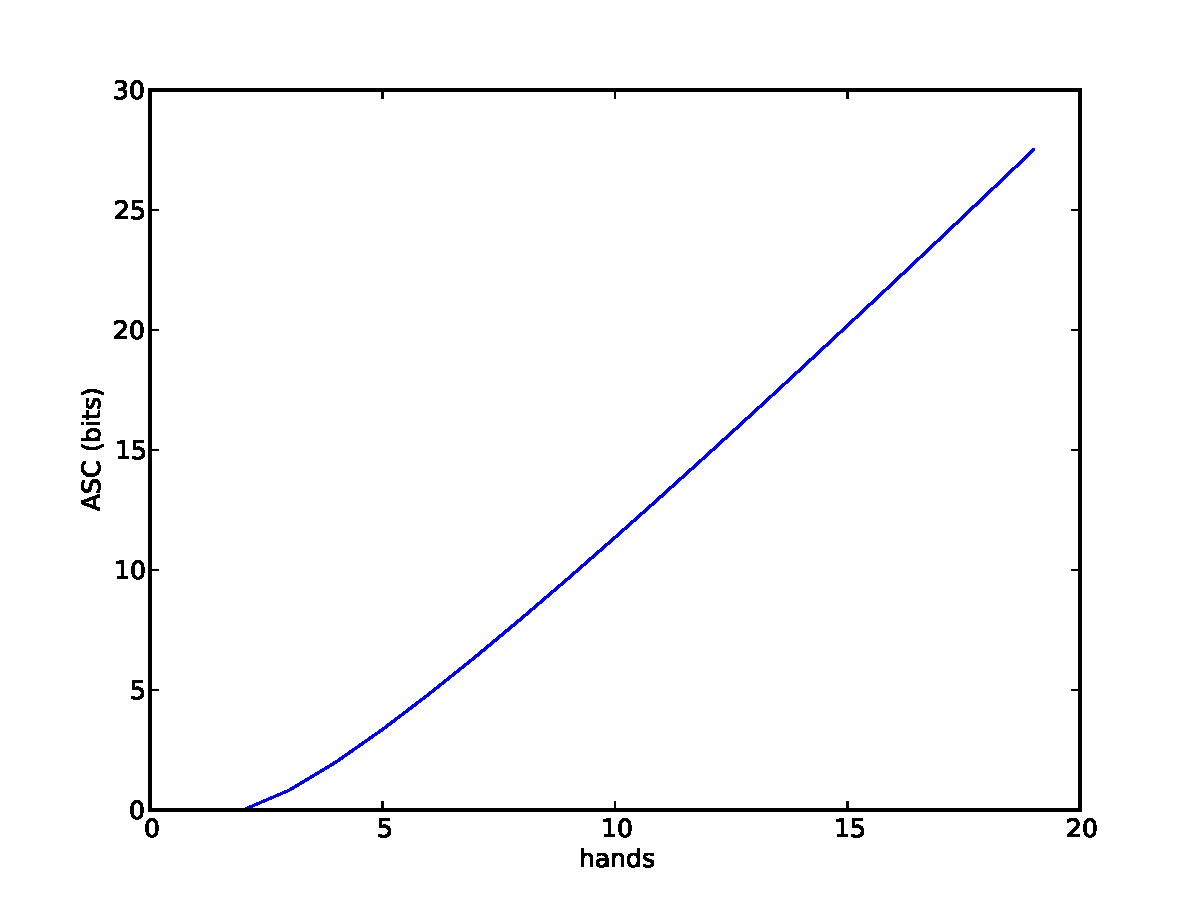
\includegraphics[width=\textwidth]{EwertRepeat}
    \caption{A plot of ASC for getting the same suit repeatedly}
    \label{suit.plot}
\end{figure}
Figure~\ref{suit.plot} shows the ASC for increasing numbers of hands.
The more times the same suit is chosen as trump, the larger the number of bits of ASC.
Given the same trump for many rounds becomes less and less probable.
\index{complexity!metrics!algorithmic specified complexity|)}

\subsection{Folding Proteins}
\label{sec_folding}

\index{proteins!folding}
In biology, an important prerequisite to a protein being functional is that it folds.
The number of all possible proteins folding has been estimated.
\begin{quotation}
    the overall prevalence of sequences performing a specific function by any domain-sized fold may be as low as 1 in $10^{77}$ \citep{axe2004}
\end{quotation}
We can create a program which outputs a particular protein, given the laws of physics.
\begin{verbatim}
for all proteins of length L
    run protein in a physics simulator
    if protein folds
        add to list of folding proteins
output the Xth protein from the list
\end{verbatim}

This program given different choices of $L$ and $N$ will output any folding protein that we choose.
This means that we can describe the protein by providing those two numbers.
\begin{equation}
    K(X|C) = 2 \log_2 L + \log_2 F_L + c
\end{equation} where $C$ is the context, in this case the law of physics.
$F_L$ is the number of folding proteins of length $L$.
Taking Axe's estimate \citep{axe2004}, an assuming simplistically, that it applies for all lengths of proteins:
\begin{equation}
    F_L = 10^{-77} 4^L 
\end{equation}
\begin{equation}
    \log F_L = -77 \log 10 + L \log 4
\end{equation}
so
\begin{equation}
    K(X|C) = 2 \log_2 L + \log_2 F_L + c = 2 \log_2 L + -77 \log 10  + L \log 4 \mbox{.}
\end{equation}

\index{DNA}\index{protein}
For our probability model, we will suppose that each base along the DNA chain is uniformly chosen.
It should be emphasized that according to the Darwinian model of evolution, the bases are not uniformly chosen.
This supposition only serves to test a simplistic chance model of protein origin.
We can calculate the probability as
\begin{equation}
    -\log_2 \Pr(X) =  -\log_2 4^{-L} = L \log_2 4 \mbox{.}
\end{equation}
Caution should be used in apply this formula.
It assumes that proportion of functional proteins is applicable for all lengths, and implies that a fractional number of proteins fold.

\index{complexity!metrics!algorithmic specified complexity}
Finally calculating the ASC,
\begin{align}
    ASC(X,p) &= L \log 4 - 2 \log_2 L + 77 \log_2 10 - L \log_2 4 - c \nonumber \\
    &= - 2 \log_2 L + 77 \log_2 10 - c \mbox{.}
\end{align}
The final bound for ASC depends little on the length of the protein sequence which only comes to play in the logarithmic term.
The significant term is the $77 \log_2 10 \approx 255.79 \mbox{ bits}$.
This means that we have good reason to believe that folding sequences were not generated randomly from a uniform distribution.

\subsection{Functional Sequence Complexity}
\index{functional sequence complexity|see{complexity, metrics, functional sequence complexity}}
\index{complexity!metrics!functional sequence complexity|(}
\index{complexity!metrics!algorithmic specified complexity|(}
Kirk Durston {\it et. al.} have defined the idea of {\it functional sequence complexity} \citep{Durston2007}.
Functional sequence complexity is related to a special case of algorithmic specified complexity.

A protein is made from a sequence of amino acids.
Some sequences have functionality and some do not.
The case considered in section \ref{sec_folding} above of folding is one particular case.
But perhaps more interesting is considering the case of various proteins which perform useful biological functions.

Let $\Omega$ be the set of all proteins.
Let $F$ be the set of all proteins which pass a functionality test.
Let $f(x)$ be a probability distribution over $F$.
Both $F$ and $f(x)$ can be produced by a simple algorithm using a functionality test on each element of $\Omega$.
Consequently, $F$ and $f(x)$ can be described using a constant program length.

Consider the average for ASC over all elements in $F$.
\begin{align}
    \label{ASC.FSC.1}
    \sum_{x \in F} f(x) A(x,C,p) 
    &= \sum_{x \in F} f(x) (-\log p(x) - K(x|C))  \nonumber \\
    &= \sum_{x \in F} -f(x)\log p(x) - \sum_{x in F} f(x) K(x|C))
\end{align}

We can describe any element $x$ given the probability distribution and $\log f(x) \mbox{ bits}$.
Given that we can calculate $f(x)$ and $F$ with a constant program gives:
\begin{equation}
    K(x|C) \leq \log -f(x) + c  \mbox{.}
\end{equation}
Place this into equation~\ref{ASC.FSC.1}.
\begin{equation}
    \sum_{x \in F} f(x) A(x,C,p) 
    \geq \sum_{x \in F} -f(x)\log p(x) - \sum_{x \in F} - f(x) \log f(x) - \sum_{x \in F} c
\end{equation}
The middle term is recognized as the Shannon entropy.
\begin{equation}
    \sum_{x \in F} f(x) A(x,C,p) 
    \geq \sum_{x \in F} -f(x) \log p(x) - H(f) - c \sum_{x \in F} f(x)
\end{equation}
If we assume that the distribution $p$ is uniform, $p(x) = \frac{1}{|\Omega|}$,
\begin{equation}
    \sum_{x \in F} f(x) A(x,C,p) 
    \geq \log_2 |\Omega| \sum_{x \in F} f(x) - H(f) - c \sum_{x \in F} f(x)  \mbox{.}
\end{equation}
The two summations over F, are summations over a probability distribution and therefore 1.
\begin{equation}
    \sum_{x \in F} f(x) A(x,C,p) 
    \geq \log_2 |\Omega| - H(f) - c 
\end{equation}
Equation 5 in Durston's work, adjusting for notation is
\begin{equation}
    \log |\Omega| - H(f)  \mbox{.}
\end{equation}
This equation derives from making the same uniformity assumption that we have made here.
Thus, for the uniform probability distribution case,
\begin{equation}
    \sum_{x \in F} (f(x) A(x,C,p) ) + c
    \geq \log |\Omega| - H(f)  \mbox{.}
\end{equation}
This establishes the relationship between ASC and FSC.
The difference is that the ASC is a lower bound, and includes a constant.
This is the same constant as elsewhere: the length of the program required to describe the specification.
\index{complexity!metrics!functional sequence complexity|)}
\index{complexity!metrics!algorithmic specified complexity|)}

\section{Objections}

\subsection{Natural Law}
\index{natural law}
\index{compressibility}
\index{information}
We have argued that compressibility in the presence of context is a necessary condition for information.
This is in contrast to other who have argued that lack of compressibility is a necessary condition for information \citep{Abel2005}.
But compressible objects lack complexity.
Because a compressible object is describable as some simple pattern, it is amenable to being produced by a simple process.
Many objects in the real world follow simple patterns.
Water tends to collect at lower elevations.
Beaches follow a slopping pattern.
Sparks fly upwards.
But these patterns are the result of the operation of simple law-like processes.
Even if the explanations for these patterns were unknown, we would suppose due to the simplicity of the pattern shown that some simple explanation existed.

\index{redundancy}
\index{patterns}
\index{algorithms}
\index{compressibility}
The premise behind this use of compressibility is that it identifies what human would see as simple patterns.
Abel writes:
\begin{quotation}
    A sequence is compressible because it contains redundant order and patterns \citep{Abel2005}.
\end{quotation}
The problem is that algorithms are very versatile and allow the description of many patterns beyond that which humans would see as patterns.
As has been shown by the various examples in this paper, many objects which do not exhibit what humans typically identify as redundant order and patterns are in fact compressible.
Significantly, we have argued that functionality actually allows compressibility.
Contrary to what Abel states, functional sequences are compressible by virtue of the functionality they exhibit.
All of the sequences that Abel holds to be mostly incompressible are actually compressible.

But are compressible objects amenable to explanation by simple processes?
Do all compressible objects lack complexity?
If this were true, it would be problematic for algorithmic specified complexity because all specified objects would also be not complex, and no object would ever be both specified and complex.
But many compressible objects do not appear to amenable to explanation by a simple process.

As discussed, English text is compressible given a knowledge of the English language.
This does not somehow make it probable that English text will appear on a beach carved out by waves.
Ninety degree angles are very compressible; yet, they are not typically found in nature.
The existence of an explanation from the laws of nature does not appear to follow from compressibility.

\index{complexity!metrics!Kolmogorov complexity}
Kolmogorov complexity deliberately ignores how long a program takes to run.
It is only concerned with the length of the program's description.
A program may be short but take an astronomical amount of time to run.
Many of the specifications considered in this paper fall into that category.
These objects are compressible, but that compression does not give an practical way to reproduce the object.
But if there is no practical way to reproduce the object, we have no reason to suggest law-like processes as a plausible explanation.

\subsection{Context is Subjective}
\index{context}\index{subjectivity}
The ASC of any object will depend on the context chosen.
Any object can be made to have high ASC by using a specifically chosen context.
But this appears to be the way that information works.
If the authors, who do not understand Arabic, look at Arabic text, it appears to be no better then scribbling.
The problem is not that Arabic lacks information content, but that we are unable to identify it without the necessary context.
As a result, this subjectivity appears to capture something about the way information works in the human experience.

\index{specification}
As with specification, it is important the context be chosen independent of object under investigation.
While a specification will rarely be independent of the object under investigation, we believe it is much easier to maintain this independence in the case of a context.

\subsection{Incalculability}
\index{incomputability}
It is not possible to calculate the Kolmogorov complexity of an object.
However, it is possible to upper bound the Kolmogorov complexity and thus lower-bound the algorithmic specified complexity.
This means that we can say that something is at least this specified, although we cannot rule out the possibility that it is even more specified.
This means that we cannot mechanically detect that something has specification, although we can objectively identify it when we see it.

\section{Conclusions}

\index{complexity!metrics!specified complexity}
\index{complexity!metrics!algorithmic specified complexity}
Dembski argued that information can be detected by looking for specified complexity.
We propose that all or most forms of specification can be represented as algorithms, using Kolmogorov complexity.
The shorter the algorithm, the more specified the object is.
In order to measure a broader range of specification, we include the context and thus make use of conditional Kolmogorov complexity.
We have defined the concept of Algorithmic Specified Complexity which takes into account the probabilistic complexity as well as the Kolmogorov complexity. 
We have presented a number of examples showing how this can represent the specification in a variety of cases.
We hope that this paper introduces discussion on the use of conditional Kolmogorov complexity as a method for measuring specification as well as the use of Algorithmic Specified Complexity.

\unnumberednotocsection{Acknowledgements}{Acknowledgements}

The approach of using compressibility as a measurement of specification was suggested to the authors by Eric Holloway.
We have attempted to extend the approach to apply to many more types of specifications.
We are grateful for his initial suggestion and answer to our initial objections to the idea.

\eandmbibliography{EwertLibrary}
